\documentclass[9pt]{beamer}
\mode<presentation>
\usepackage[T1]{fontenc}
\usepackage{color}
\usepackage{graphicx}
\usepackage{natbib}
\usepackage{tikz}
\usetikzlibrary{shapes.geometric}
\usepackage{xmpmulti}
\usepackage{animate}
\usepackage{tcolorbox}
\usepackage{amsmath}
\usepackage{gensymb}
\usepackage{csquotes}
\usepackage{bibentry}
\nobibliography*

\usetheme{Singapore}
%\usecolortheme{seahorse}

\usefonttheme{professionalfonts}

\title[Word \& Doc Embeddings]{A Rapid Computer-assisted Systematic Map of Regional Climate Impacts}
%\author{Max Callaghan, Gerritt }
\institute[MCC]{
	
\includegraphics[height=1cm,width=2cm]{images/MCC_Logo_RZ_rgb.jpg} \hspace{5em} 
\includegraphics[height=1cm]{images/climate_analytics.png}
}

\newif\ifframeinlbf
\frameinlbftrue
\makeatletter
\newcommand\listofframes{\@starttoc{lbf}}
\makeatother

\addtobeamertemplate{frametitle}{}{%
	\ifframeinlbf
	\addcontentsline{lbf}{section}{\protect\makebox[2em][l]{%
			\protect\usebeamercolor[fg]{structure}\insertframenumber\hfill}%
		\insertframetitle\par}%
	\else\fi
}

\newtheorem*{remark}{}

\bibliographystyle{apalike}

\begin{document}
	
\begin{frame}
	\titlepage
\end{frame}

\begin{frame}{Outline}

\tableofcontents

\end{frame}

\section{Introduction}

\begin{frame}{Context}

Systematic assessments of the evidence on Climate Change like those conducted by the IPCC are vital.

\begin{columns}
	\begin{column}{0.618\linewidth}
		\begin{figure}
			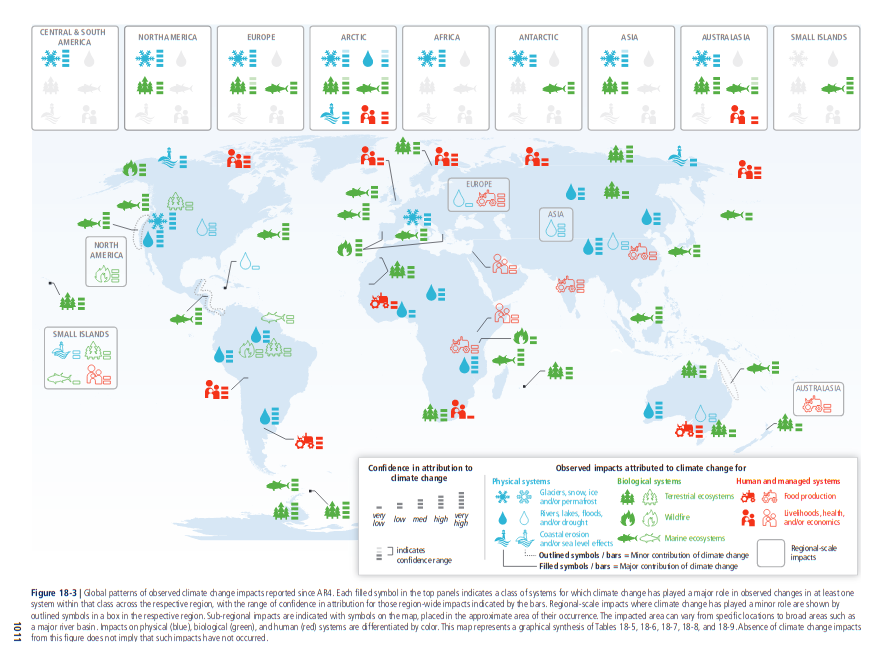
\includegraphics[width=\linewidth]{../map_18.png}<1->
		\end{figure}
	\end{column}
	\begin{column}{0.312\linewidth}
		
		\begin{figure}
			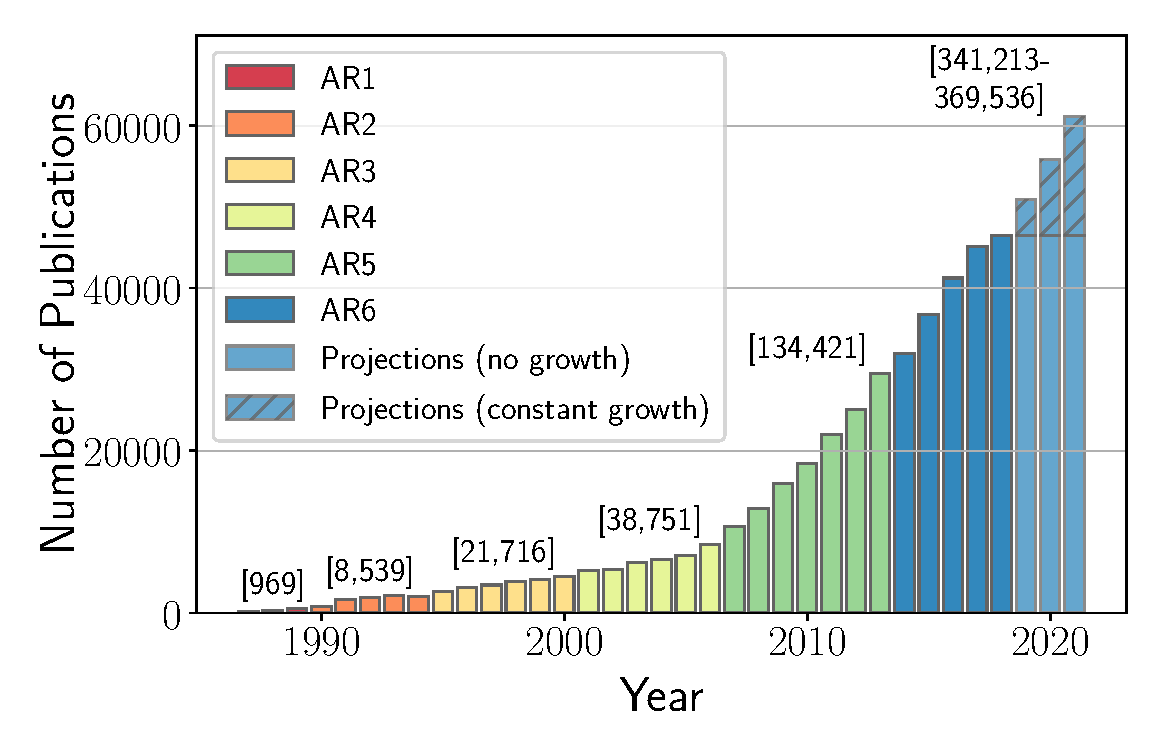
\includegraphics[width=\linewidth]{images/pubs_time_wgb_lp.pdf}<2->
		\end{figure}
		
		\begin{itemize}
			\small
			\item<2->These are challenged by big literature 
			\item<3->They do not account for uncertainty about what literature is available
		\end{itemize}
	\end{column}
\end{columns}

\end{frame}

\begin{frame}{Goal}
There are hundreds of thousands of documents potentially relevant to observed climate impacts. We want to be able to do two things:

\begin{itemize}
	\item<2-> Separate those documents which \textit{are} relevant from those that are not
	\item<3-> Predict in what way relevant documents are relevant:
	\begin{itemize}
		\item What impacts do they document?
		\item What type of evidence do they provide?
		\item In which locations is there evidence
	\end{itemize}
\end{itemize}

\only<4->{Once we can do that, we can draw a rough map of the available evidence, and/or aid the production of an \textit{assessment} of the available evidence}

\end{frame}



\begin{frame}{Distribution of labour between humans and machines}

A human expert or a team of human experts is best placed to answer those questions for any single document, but they can't look at all potentially relevant documents

\bigskip

We can use labels generated by humans to try to teach a computer what a relevant document looks like, and how to decide in what way it is relevant. 

\bigskip

If this works well, we can predict, with some uncertainty, how much evidence there is, and where and on what topic it is.

\end{frame}

\section{Data collection}
\begin{frame}
\tableofcontents[currentsection]
\end{frame}

\begin{frame}{We set up our platform to record the relevance and lots of other information about each document}

\begin{figure}
	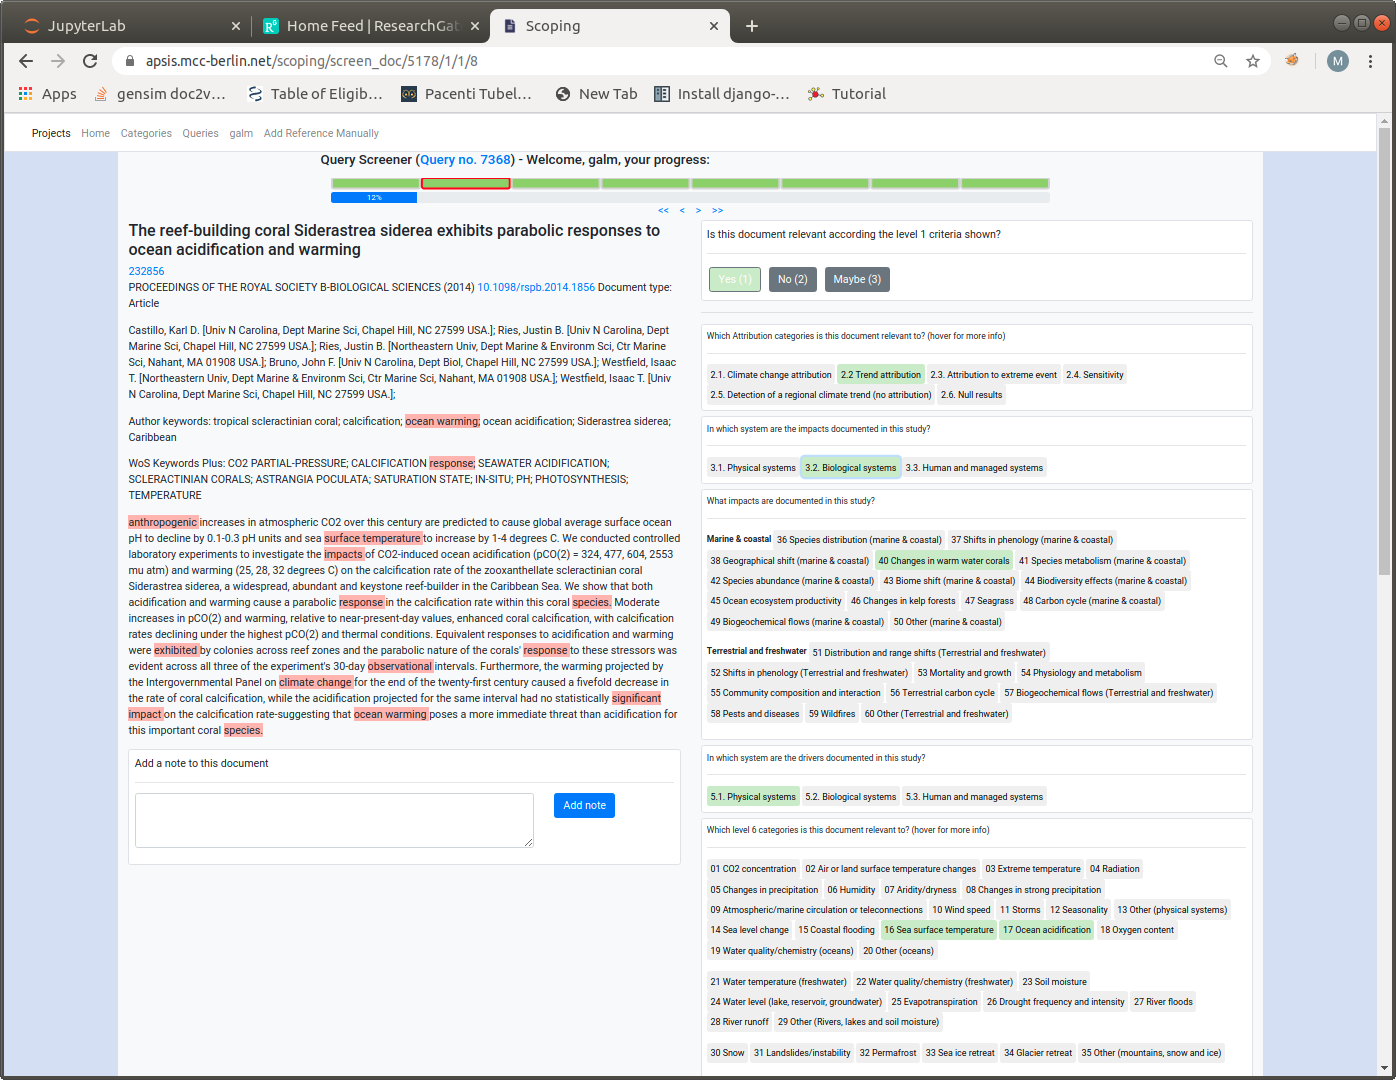
\includegraphics[width=\linewidth]{../plots/screening-platform}
\end{figure}

\end{frame}

\begin{frame}{During the first couple of months of lockdown we screened 1500 documents}

\begin{figure}
	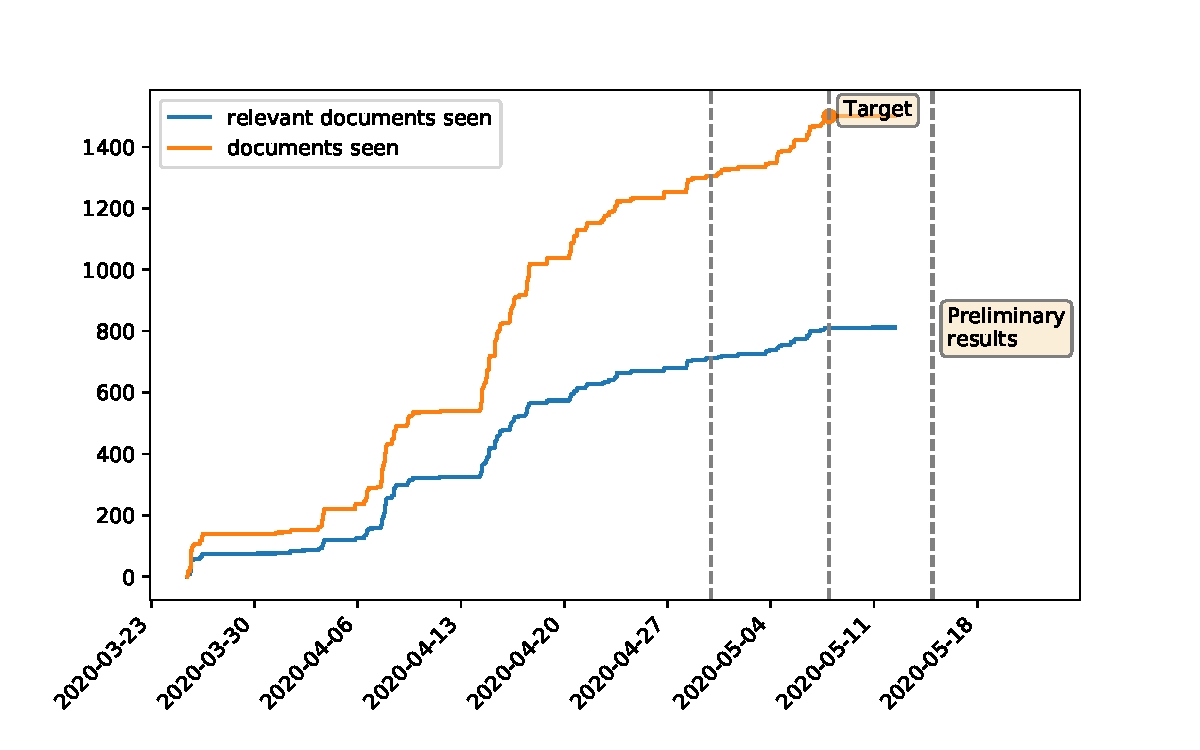
\includegraphics[width=\linewidth]{../plots/progress/plan.pdf}
\end{figure}

\end{frame}

\begin{frame}{This already constitutes a useful information gathering exercise}

\begin{figure}
	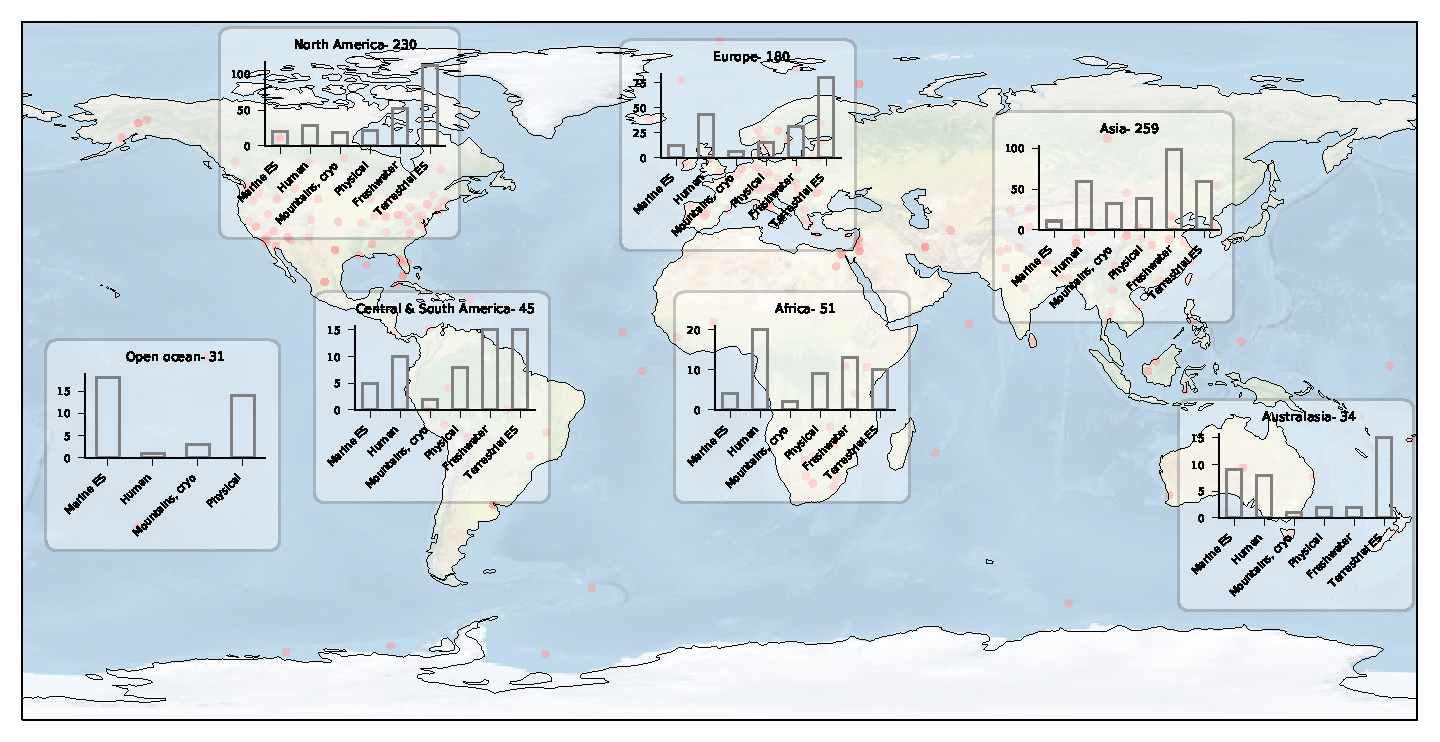
\includegraphics[width=\linewidth]{../plots/map_coded.pdf}
\end{figure}

\end{frame}

\section{Outcome 1 - Prediction Performance}
\begin{frame}
\tableofcontents[currentsection]
\end{frame}

\begin{frame}{Support Vector Machines}
\begin{columns}
	\begin{column}{0.5\linewidth}
	\begin{itemize}
		\item We train SVMs to predict binary outcomes for relevance, and for each category
		\item SVMs build a hyperplane which best separates the features of data points of different classes
		\item Our features are 1-2 word ngrams taken from the document titles and abstracts
	\end{itemize}
	\end{column}
	\begin{column}{0.5\linewidth}
	\begin{figure}
		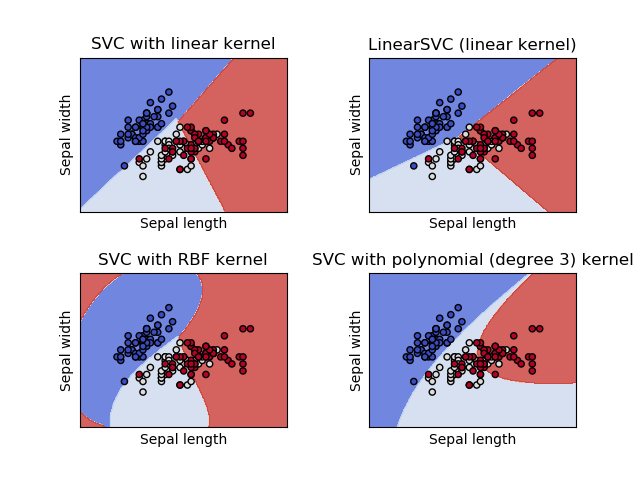
\includegraphics[width=\linewidth]{images/svc_sklearn}
		\caption{Source: \url{https://scikit-learn.org/stable/auto_examples/svm/plot_iris_svc.html}}
	\end{figure}
	\end{column}
\end{columns}

\end{frame}

%\begin{frame}{Other Data}
%
%In addition to what we collected together we also have other coded documents:
%
%\bigskip
%
%\begin{columns}[t]
%	\begin{column}{0.5\linewidth}
%		AR5 Data 256 documents we can use to supplement our training set
%	\end{column}
%	\begin{column}{0.5\linewidth}
%		700 Documents I coded earlier this year.
%		
%		500 are a random sample we can use for validation
%	\end{column}
%\end{columns}
%\end{frame}

\begin{frame}{We predict the relevance of a document most of the time}
\begin{figure}
	\begin{columns}
		\begin{column}{0.3812\linewidth}
			\begin{figure}
					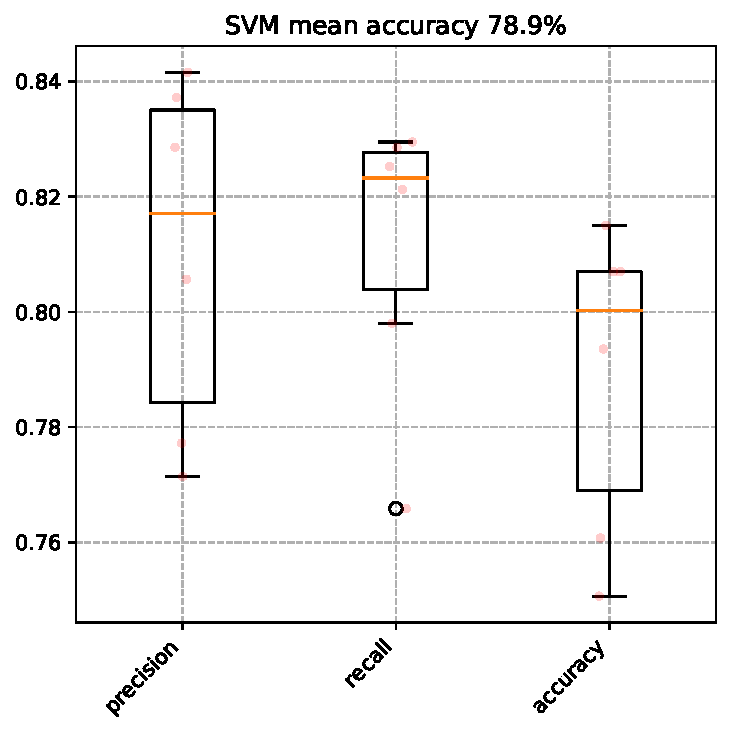
\includegraphics[width=\linewidth]{../plots/prediction_models/relevance_prediction_2020-05-12.pdf}
			\end{figure}
			\begin{figure}
				\only<1>{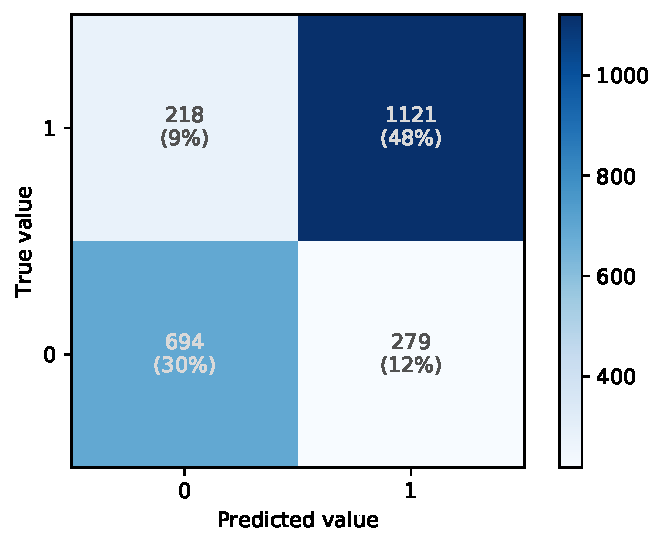
\includegraphics[width=\linewidth]{../plots/prediction_models/relevance_confusion.pdf}}
				\only<2>{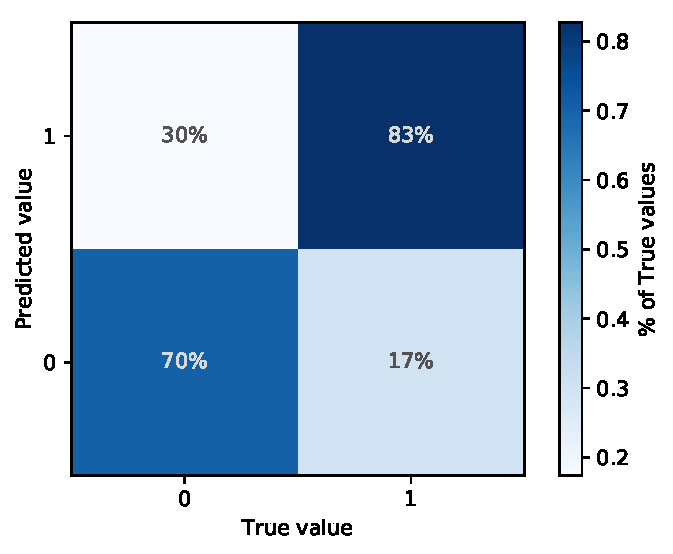
\includegraphics[width=\linewidth]{../plots/prediction_models/relevance_confusion_true.pdf}}
				\only<3>{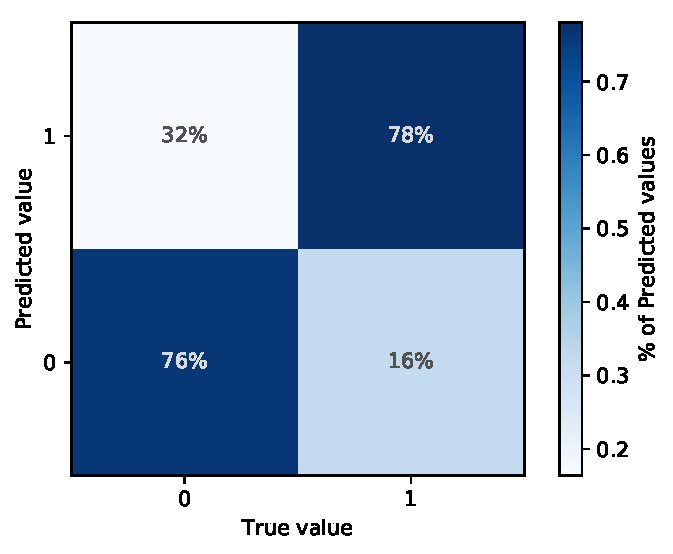
\includegraphics[width=\linewidth]{../plots/prediction_models/relevance_confusion_pred.pdf}}
			\end{figure}
		\end{column}
		\begin{column}{0.5\linewidth}
			This has been steadily increasing by using the model itself as a "second pair of eyes" to check for errors, and I expect it to increase further (partly due to different criteria for inclusion at different stages of the project)
			\only<1>{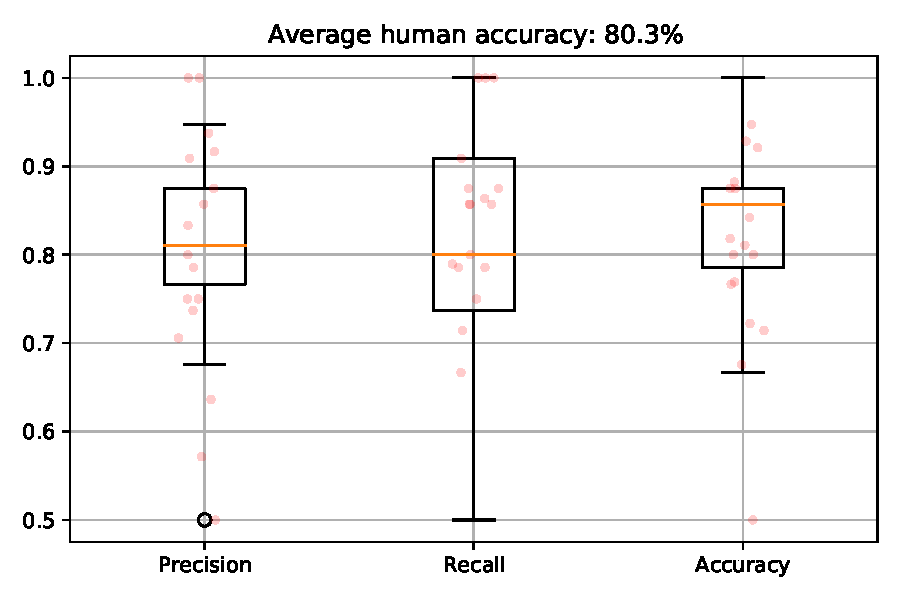
\includegraphics[width=\linewidth]{../plots/human_accuracy.pdf}}
		\end{column}
	\end{columns}

\end{figure}
\end{frame}


\begin{frame}{We can clearly identify what impact category a document is related to}

\begin{figure}
	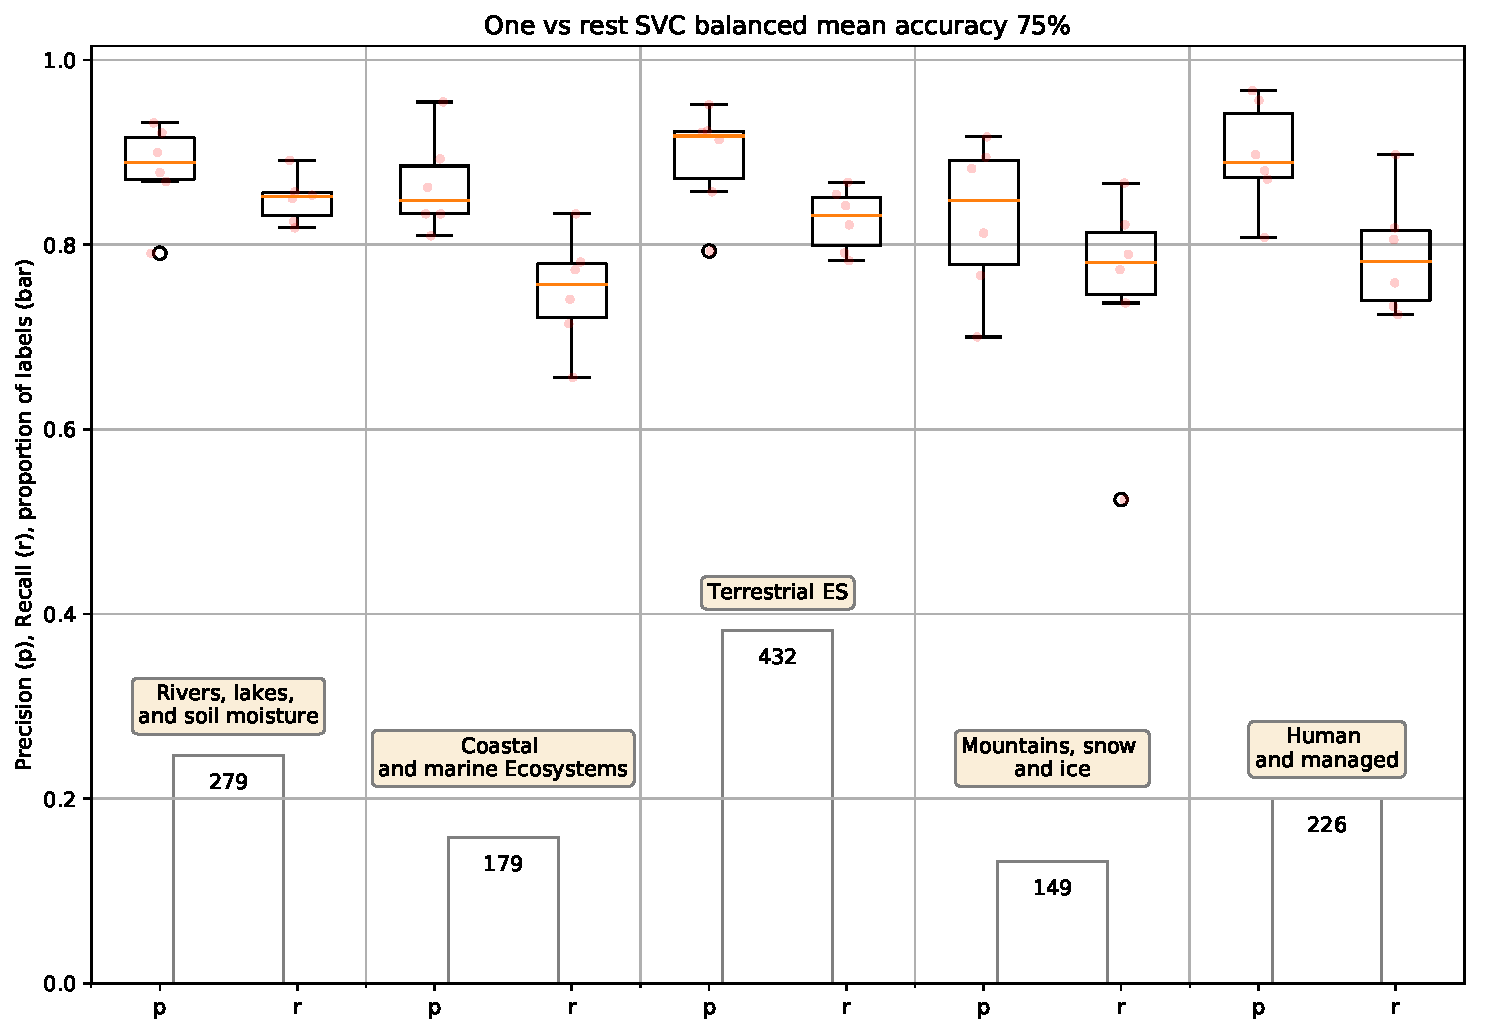
\includegraphics[width=0.9\linewidth]{../plots/progress/cats_prediction.pdf}
	\caption{Precision (how many documents predicted to be in a category actually had that label) and Recall (how many documents with a label were predicted to be in that category) for each broad impact category}
\end{figure}

\end{frame}

\begin{frame}{We can clearly identify what impact category a document is related to}

\begin{figure}
	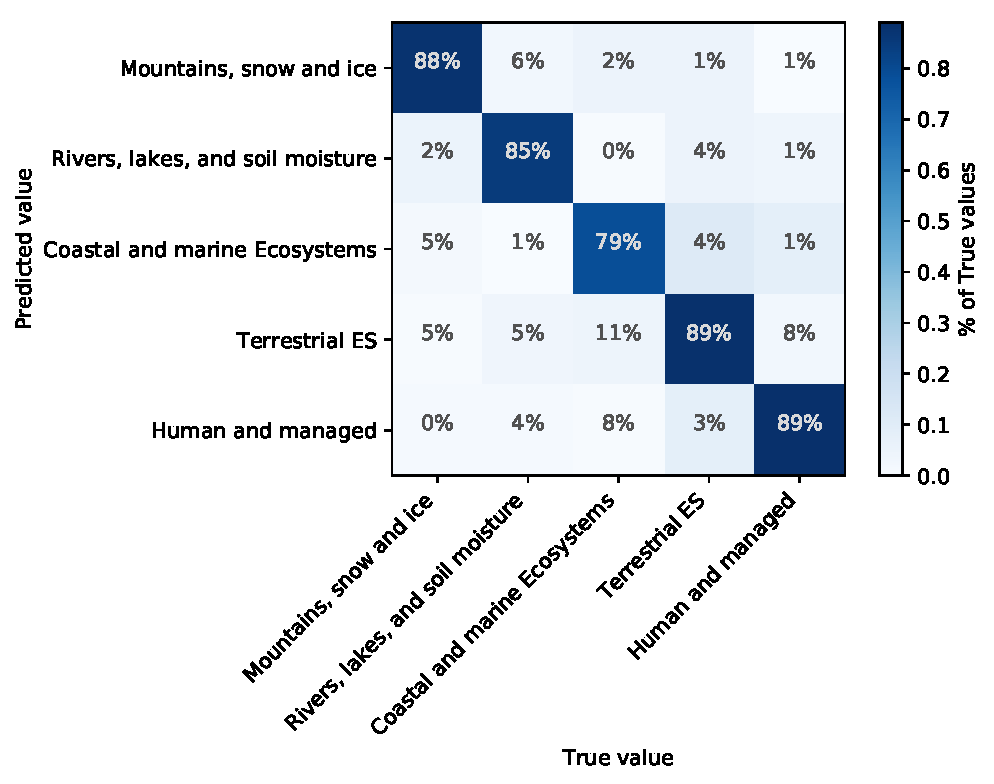
\includegraphics[width=0.9\linewidth]{../plots/prediction_models/category_confusion.pdf}
\end{figure}

\end{frame}



\begin{frame}{Accuracy increased and uncertainty decreased with the number of labels available}

\begin{figure}
	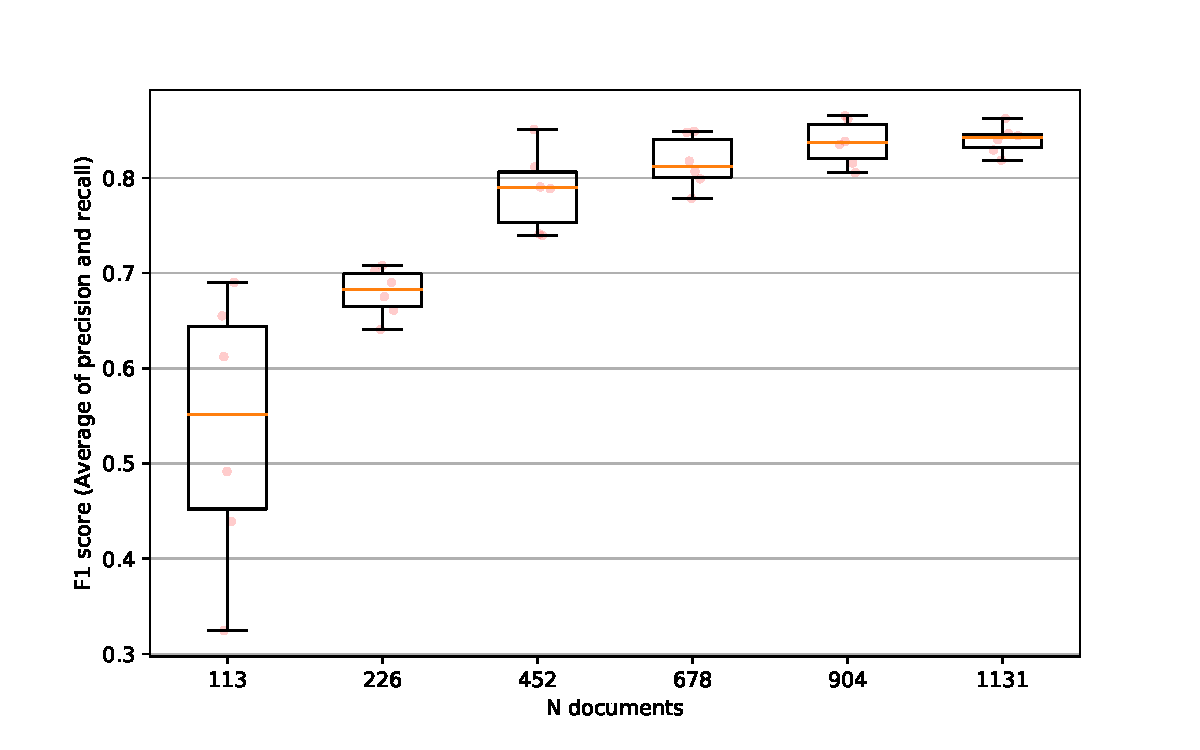
\includegraphics[width=0.8\linewidth]{../plots/progress/cats_prediction_n.pdf}

\end{figure}

\end{frame}

\begin{frame}{We are also broadly correct on subcategories - impressive given the amount of data and the complexity of the coding scheme}
	\begin{figure}
		
		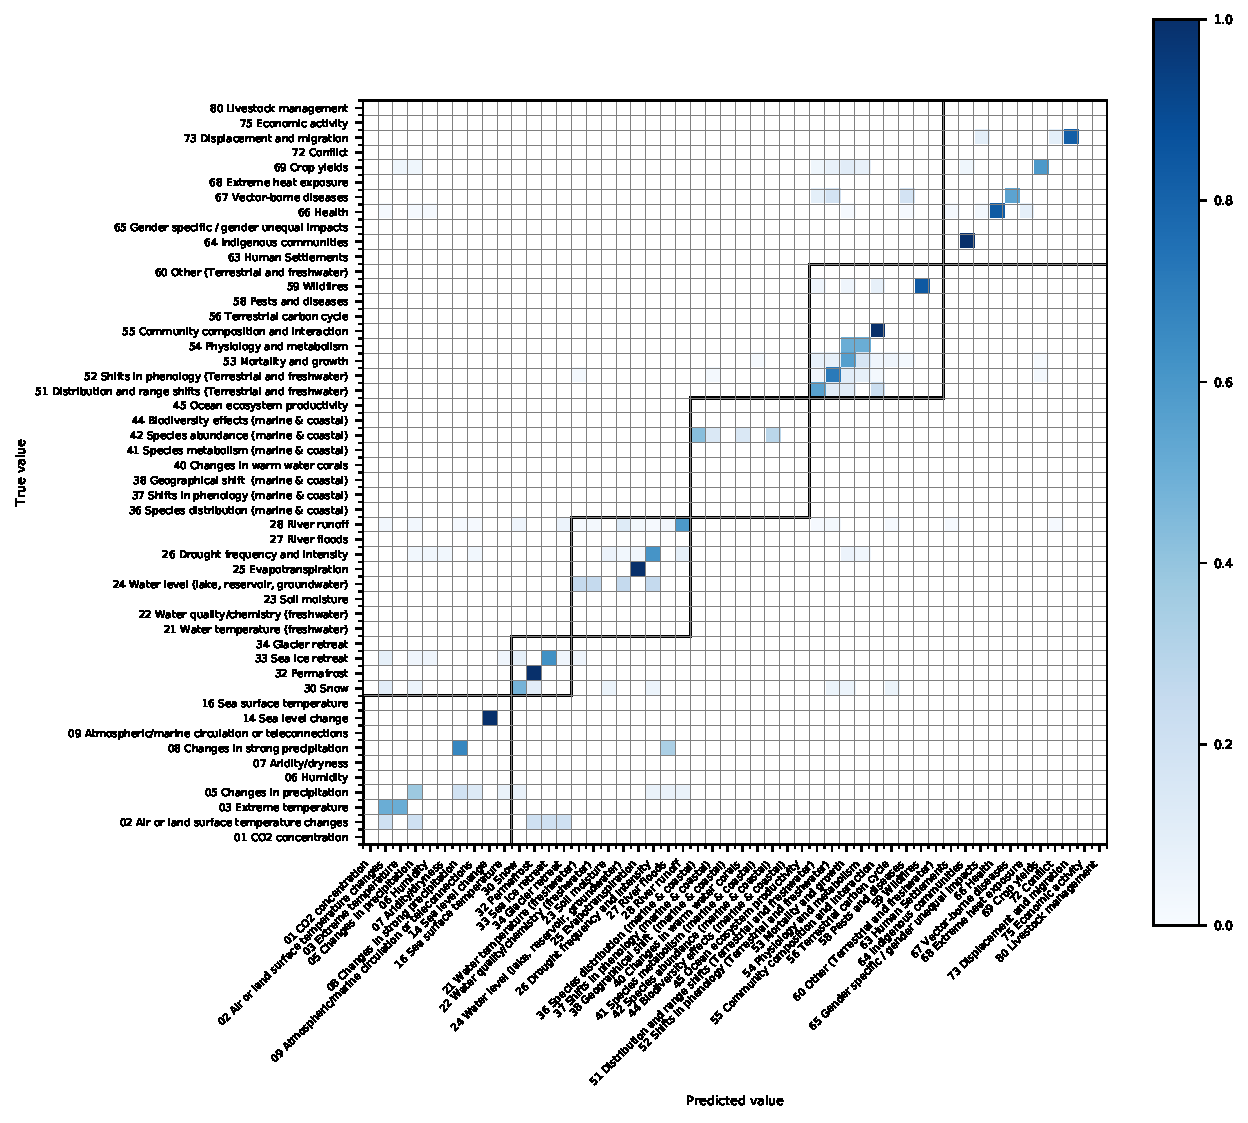
\includegraphics[width=0.8\linewidth]{../plots/prediction_models/confusion_all_classes_pred.pdf}
	\end{figure}
\end{frame}

\begin{frame}{Getting attribution correct is harder, but we have fewer labels}
	\begin{figure}
	
	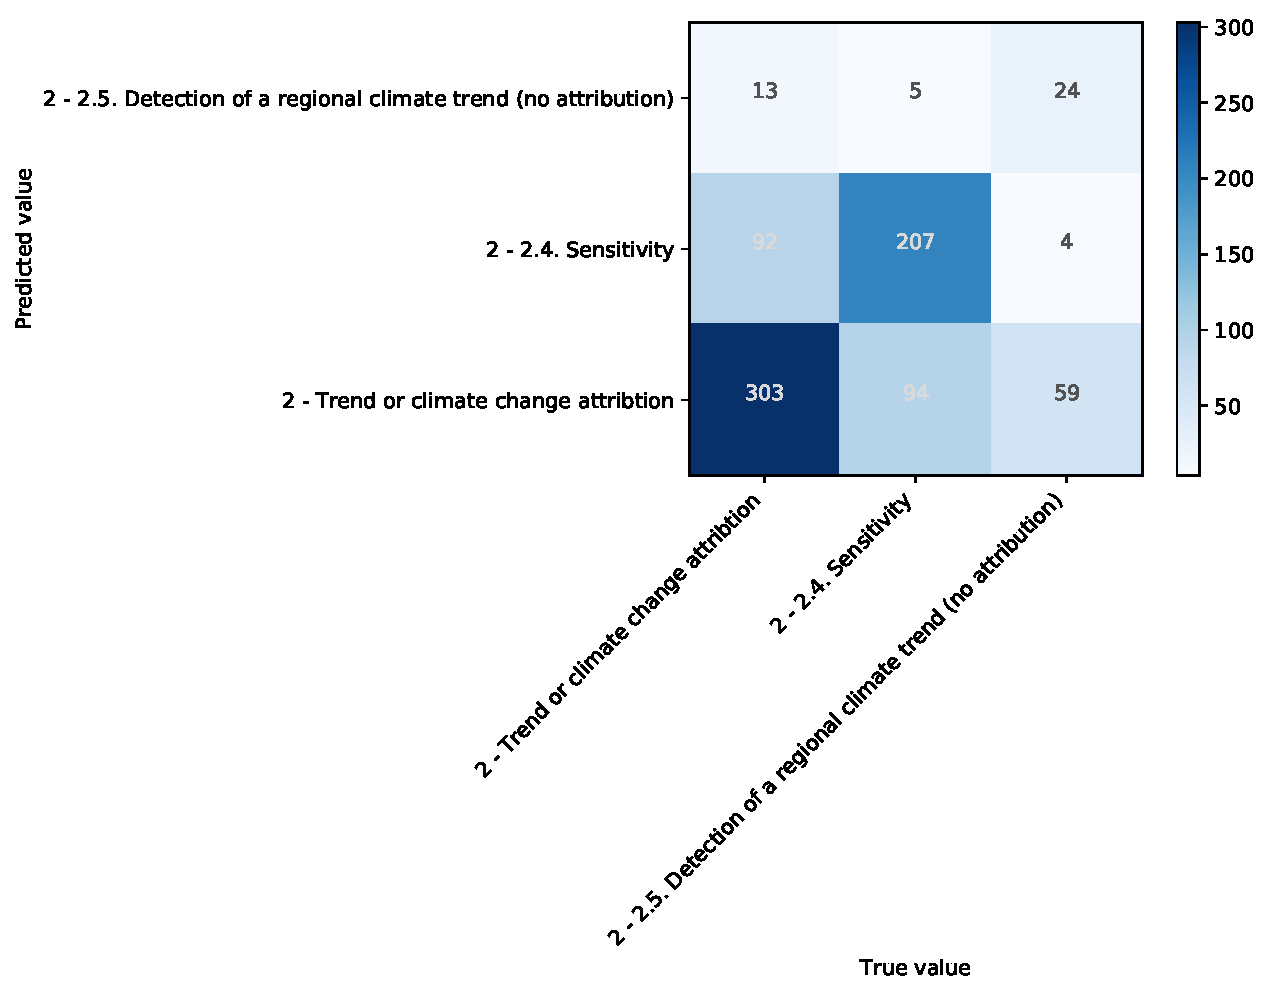
\includegraphics[width=0.8\linewidth]{../plots/prediction_models/confusion_attribution.pdf}
	\end{figure}
\end{frame}


\section{Outcome 2 - Evidence Map}
\begin{frame}
\tableofcontents[currentsection]
\end{frame}

\begin{frame}{We predict tens of thousands of additional documents relevant according to the criteria we defined}

	\begin{columns}
		\begin{column}{0.618\linewidth}
			\begin{figure}
				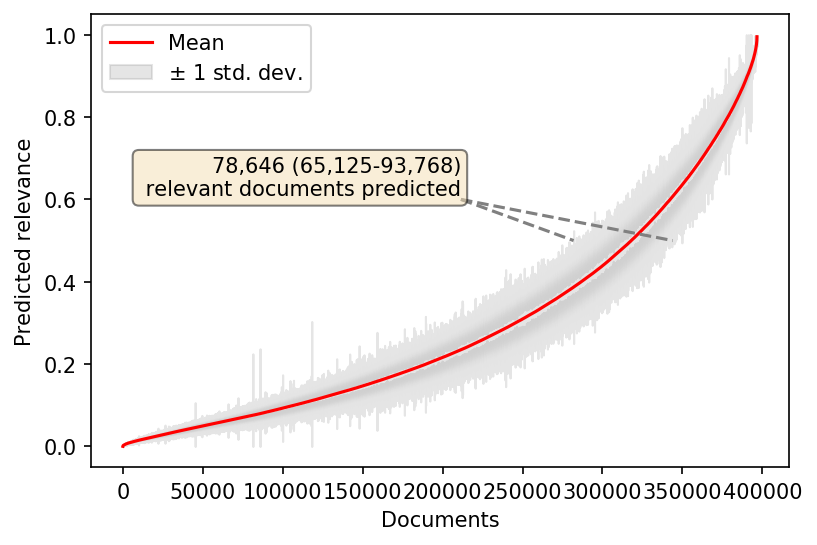
\includegraphics[width=\linewidth]{../plots/prediction_models/predictions_unseen.png}
			\end{figure}
		\end{column}
		\begin{column}{0.382\linewidth}
			\begin{itemize}
				\item We train 6 classifiers on random partitions of the labelled dataset
				\item This gives us 6 estimates for each unseen document
				\item The mean and standard deviation of these estimates give us an idea, with some uncertainty, of how many documents are in each category
				\item There must be a better way to incorporate what we know from our test statistics into our uncertainty ranges, but I can't figure it out
			\end{itemize}
		\end{column}
	\end{columns}

\end{frame}

\begin{frame}
\only<1>{
	\begin{figure}
		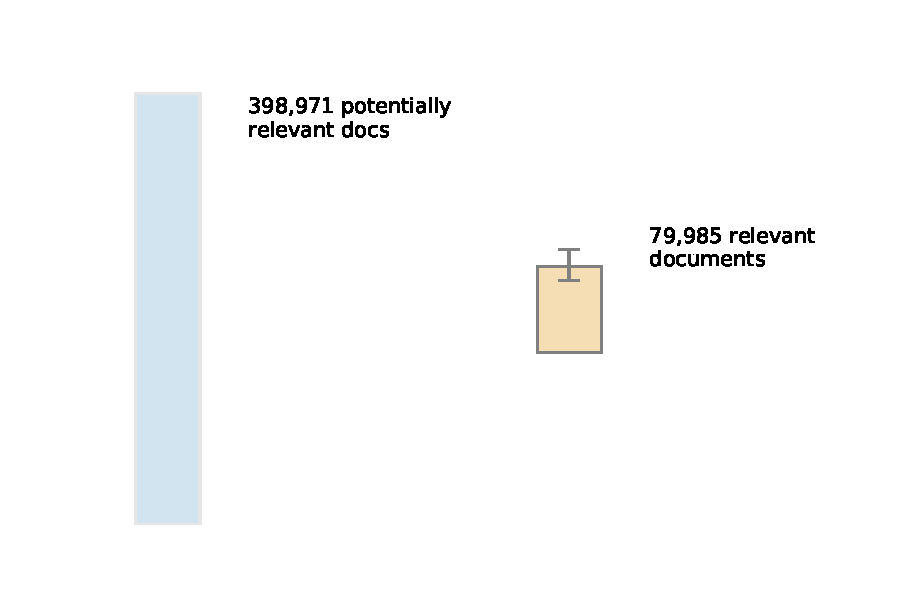
\includegraphics[width=0.7\linewidth]{../plots/process_diagram/relevant.pdf}
	\end{figure}
}
\only<2>{
	\begin{figure}
		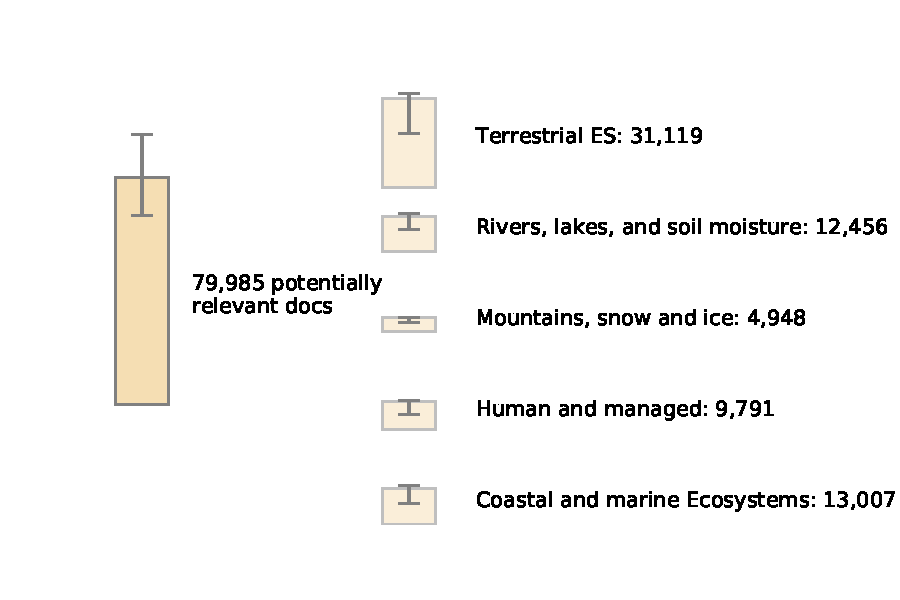
\includegraphics[width=0.7\linewidth]{../plots/process_diagram/relevant_cats.pdf}
	\end{figure}
}
\only<3>{
	\begin{figure}
		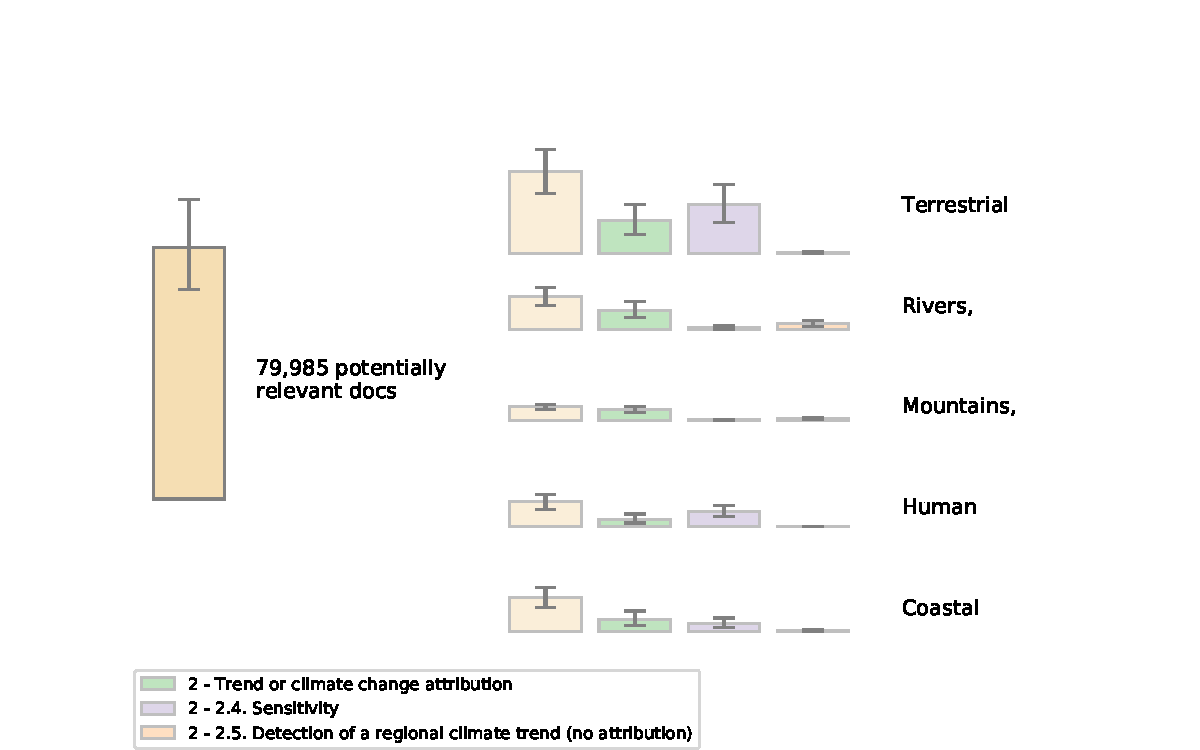
\includegraphics[width=0.7\linewidth]{../plots/process_diagram/relevant_cats_attrib.pdf}
	\end{figure}
}
\end{frame}

\begin{frame}{The studies predicted to be relevant cover a much broader array of places, but geographic imbalances persist}
\only<1>{
	\begin{figure}
	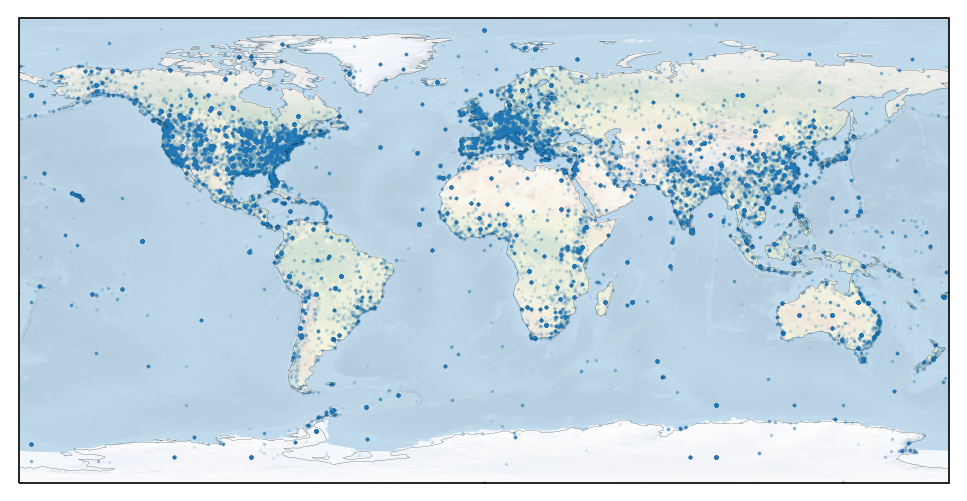
\includegraphics[width=\linewidth]{../plots/maps/all_predicted_places.png}
\end{figure}
}

\end{frame}


\begin{frame}{We have around 7,500 place names (from 3,250 unique documents predicted to have mentioned a location in Africa). These are also not evenly distributed.}
\begin{columns}
	\begin{column}{0.5\linewidth}
		\begin{figure}
			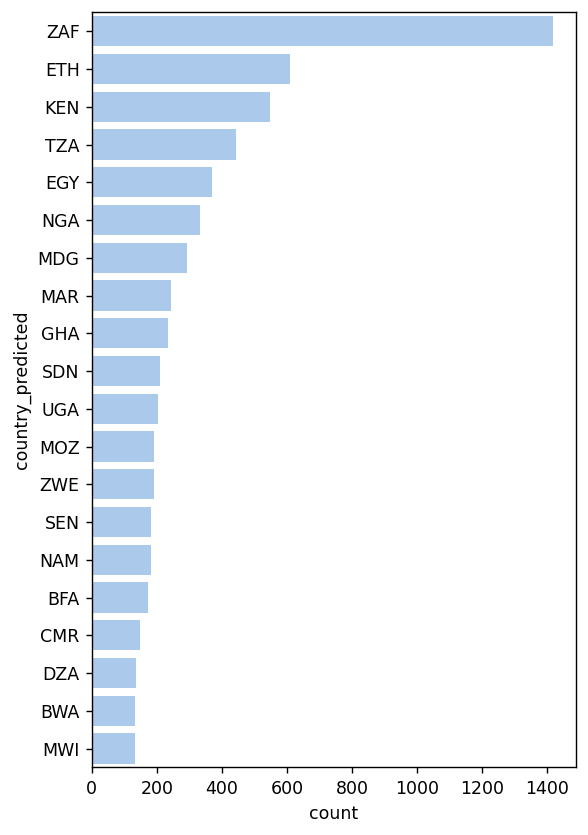
\includegraphics[width=0.8\linewidth]{../plots/literature_distribution/by_country_africa.png}
		\end{figure}
	\end{column}
	\begin{column}{0.5\linewidth}
		\begin{figure}
			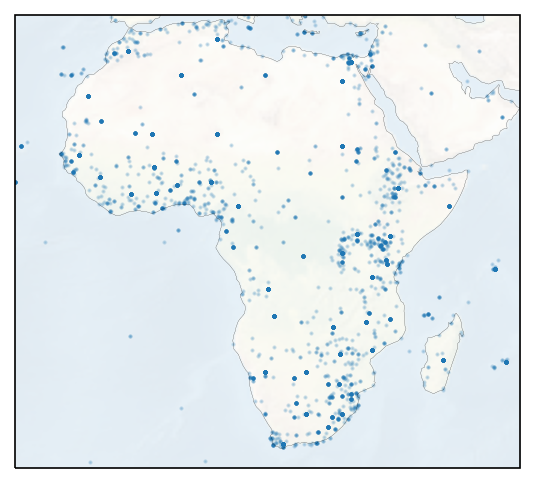
\includegraphics[width=\linewidth]{../plots/maps/predicted_places_africa.png}
		\end{figure}
	\end{column}
\end{columns}

\end{frame}


\begin{frame}{In which locations is there evidence? What impacts does it document? Since when has there been evidence?}

\begin{columns}
	\begin{column}{0.382\linewidth}
		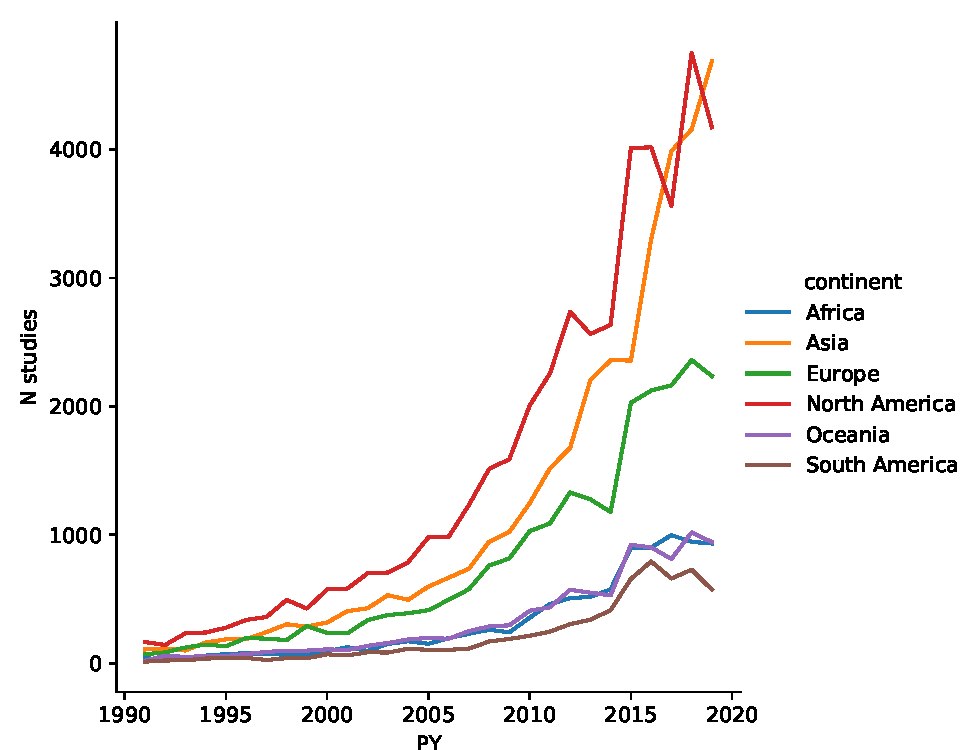
\includegraphics[width=\linewidth]{../plots/literature_distribution/PY_continent_n.pdf}
		
		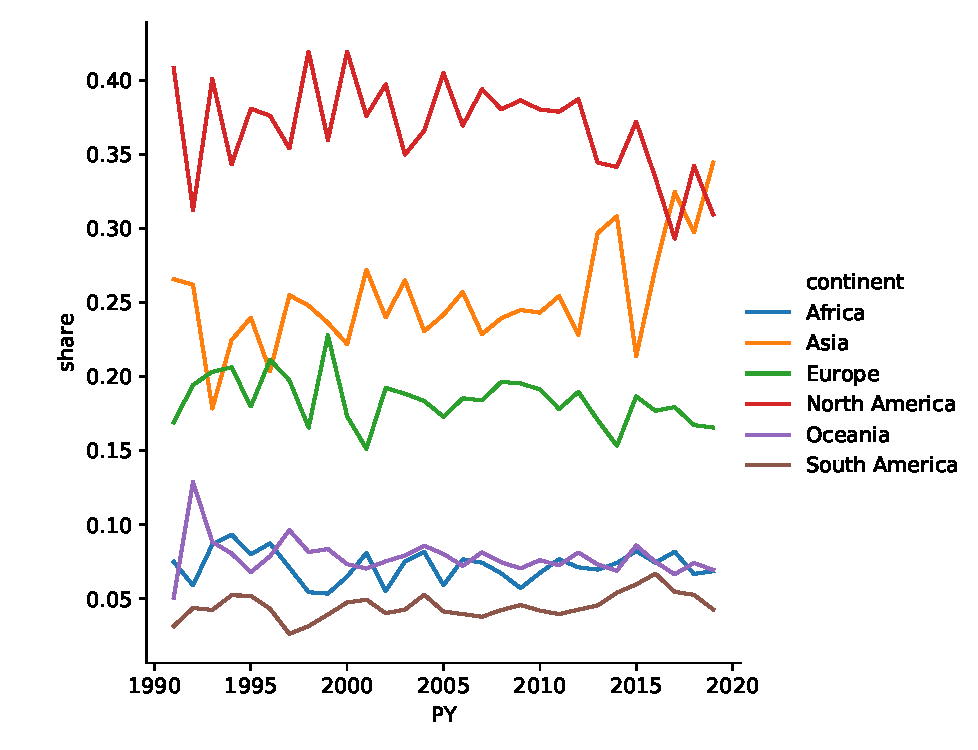
\includegraphics[width=\linewidth]{../plots/literature_distribution/PY_continent_shares.pdf}
	\end{column}
	\begin{column}{0.618\linewidth}
		\begin{itemize}
			\item More studies on Asia than North America since 2018
			\item Africa now more frequently studied than South America and Oceania
			
		\end{itemize}
	\end{column}
\end{columns}

\end{frame}

%%%

\begin{frame}{}

\begin{columns}
\begin{column}{0.382\linewidth}
	\begin{itemize}
		\item<1-> Lots of the new studies on Asia have been about Detection (is there a regional climate trend)
		\item<2-> There is also more literature on human impacts and the water cycle in Asia
		\item<3-> On human impacts, Africa is as much studied as anywhere apart from Asia
		
	\end{itemize}
\end{column}
\begin{column}{0.618\linewidth}
	\only<1->{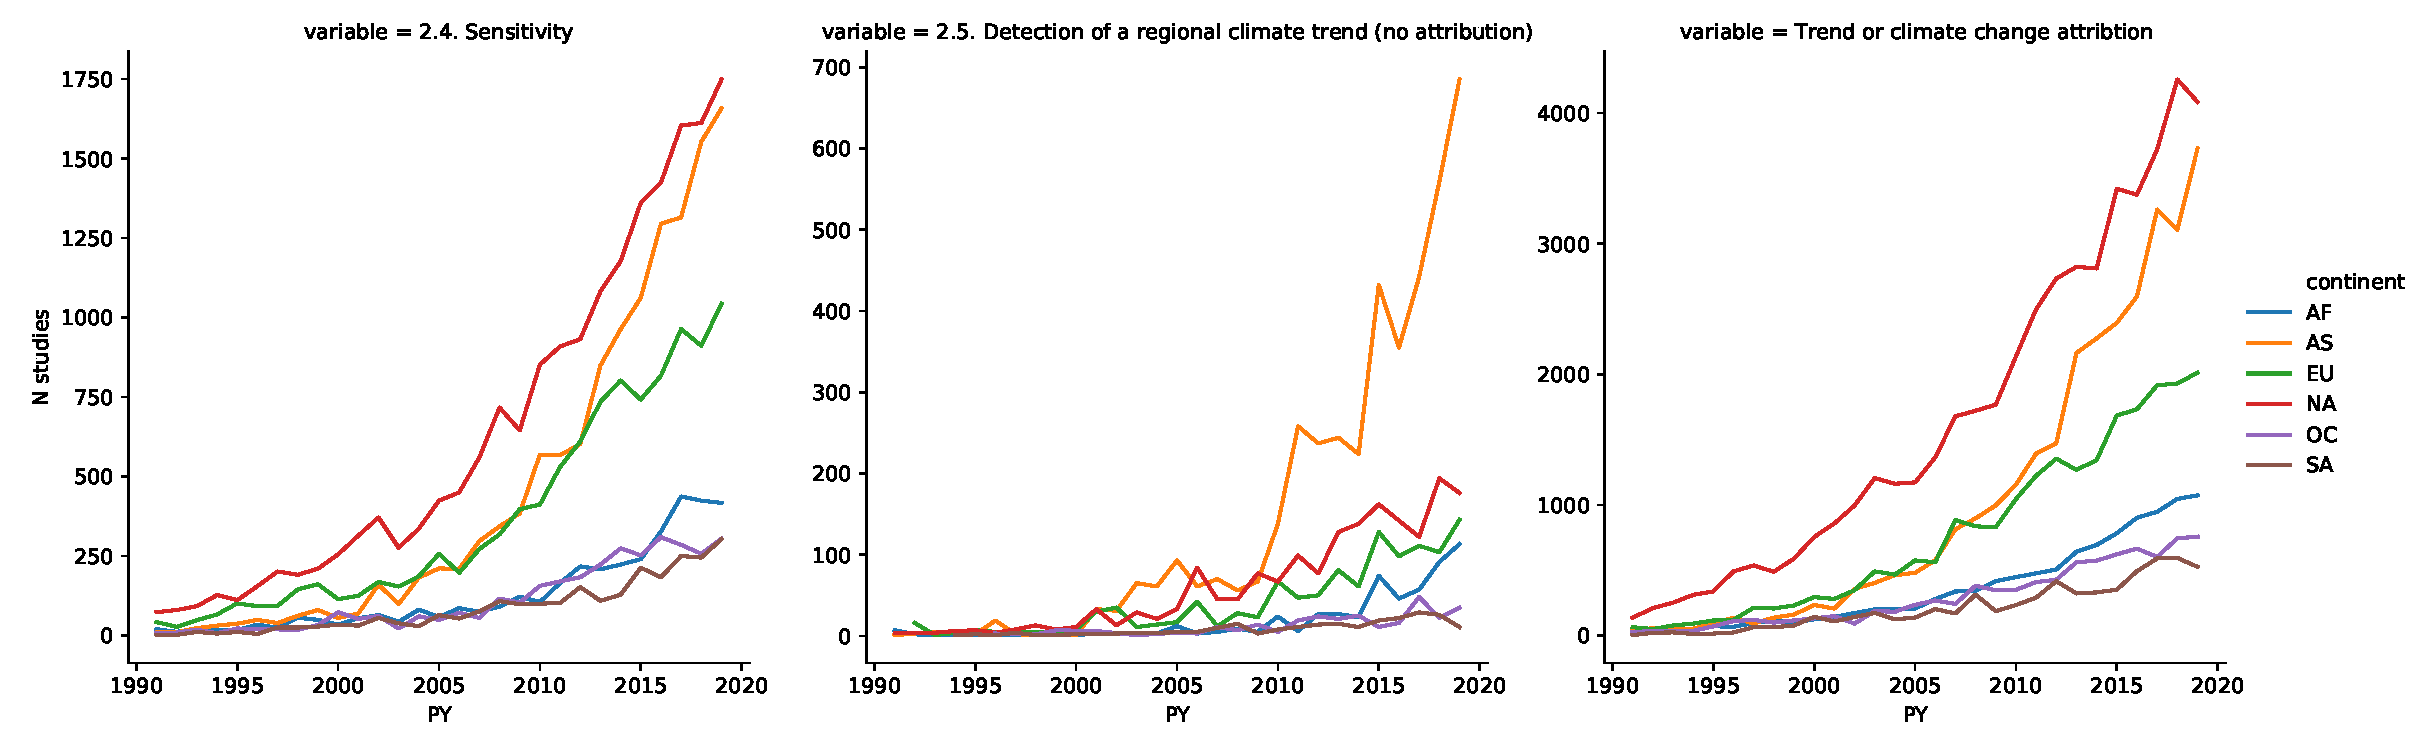
\includegraphics[width=\linewidth]{../plots/literature_distribution/PY_continent_attrib.pdf}}
	\only<2->{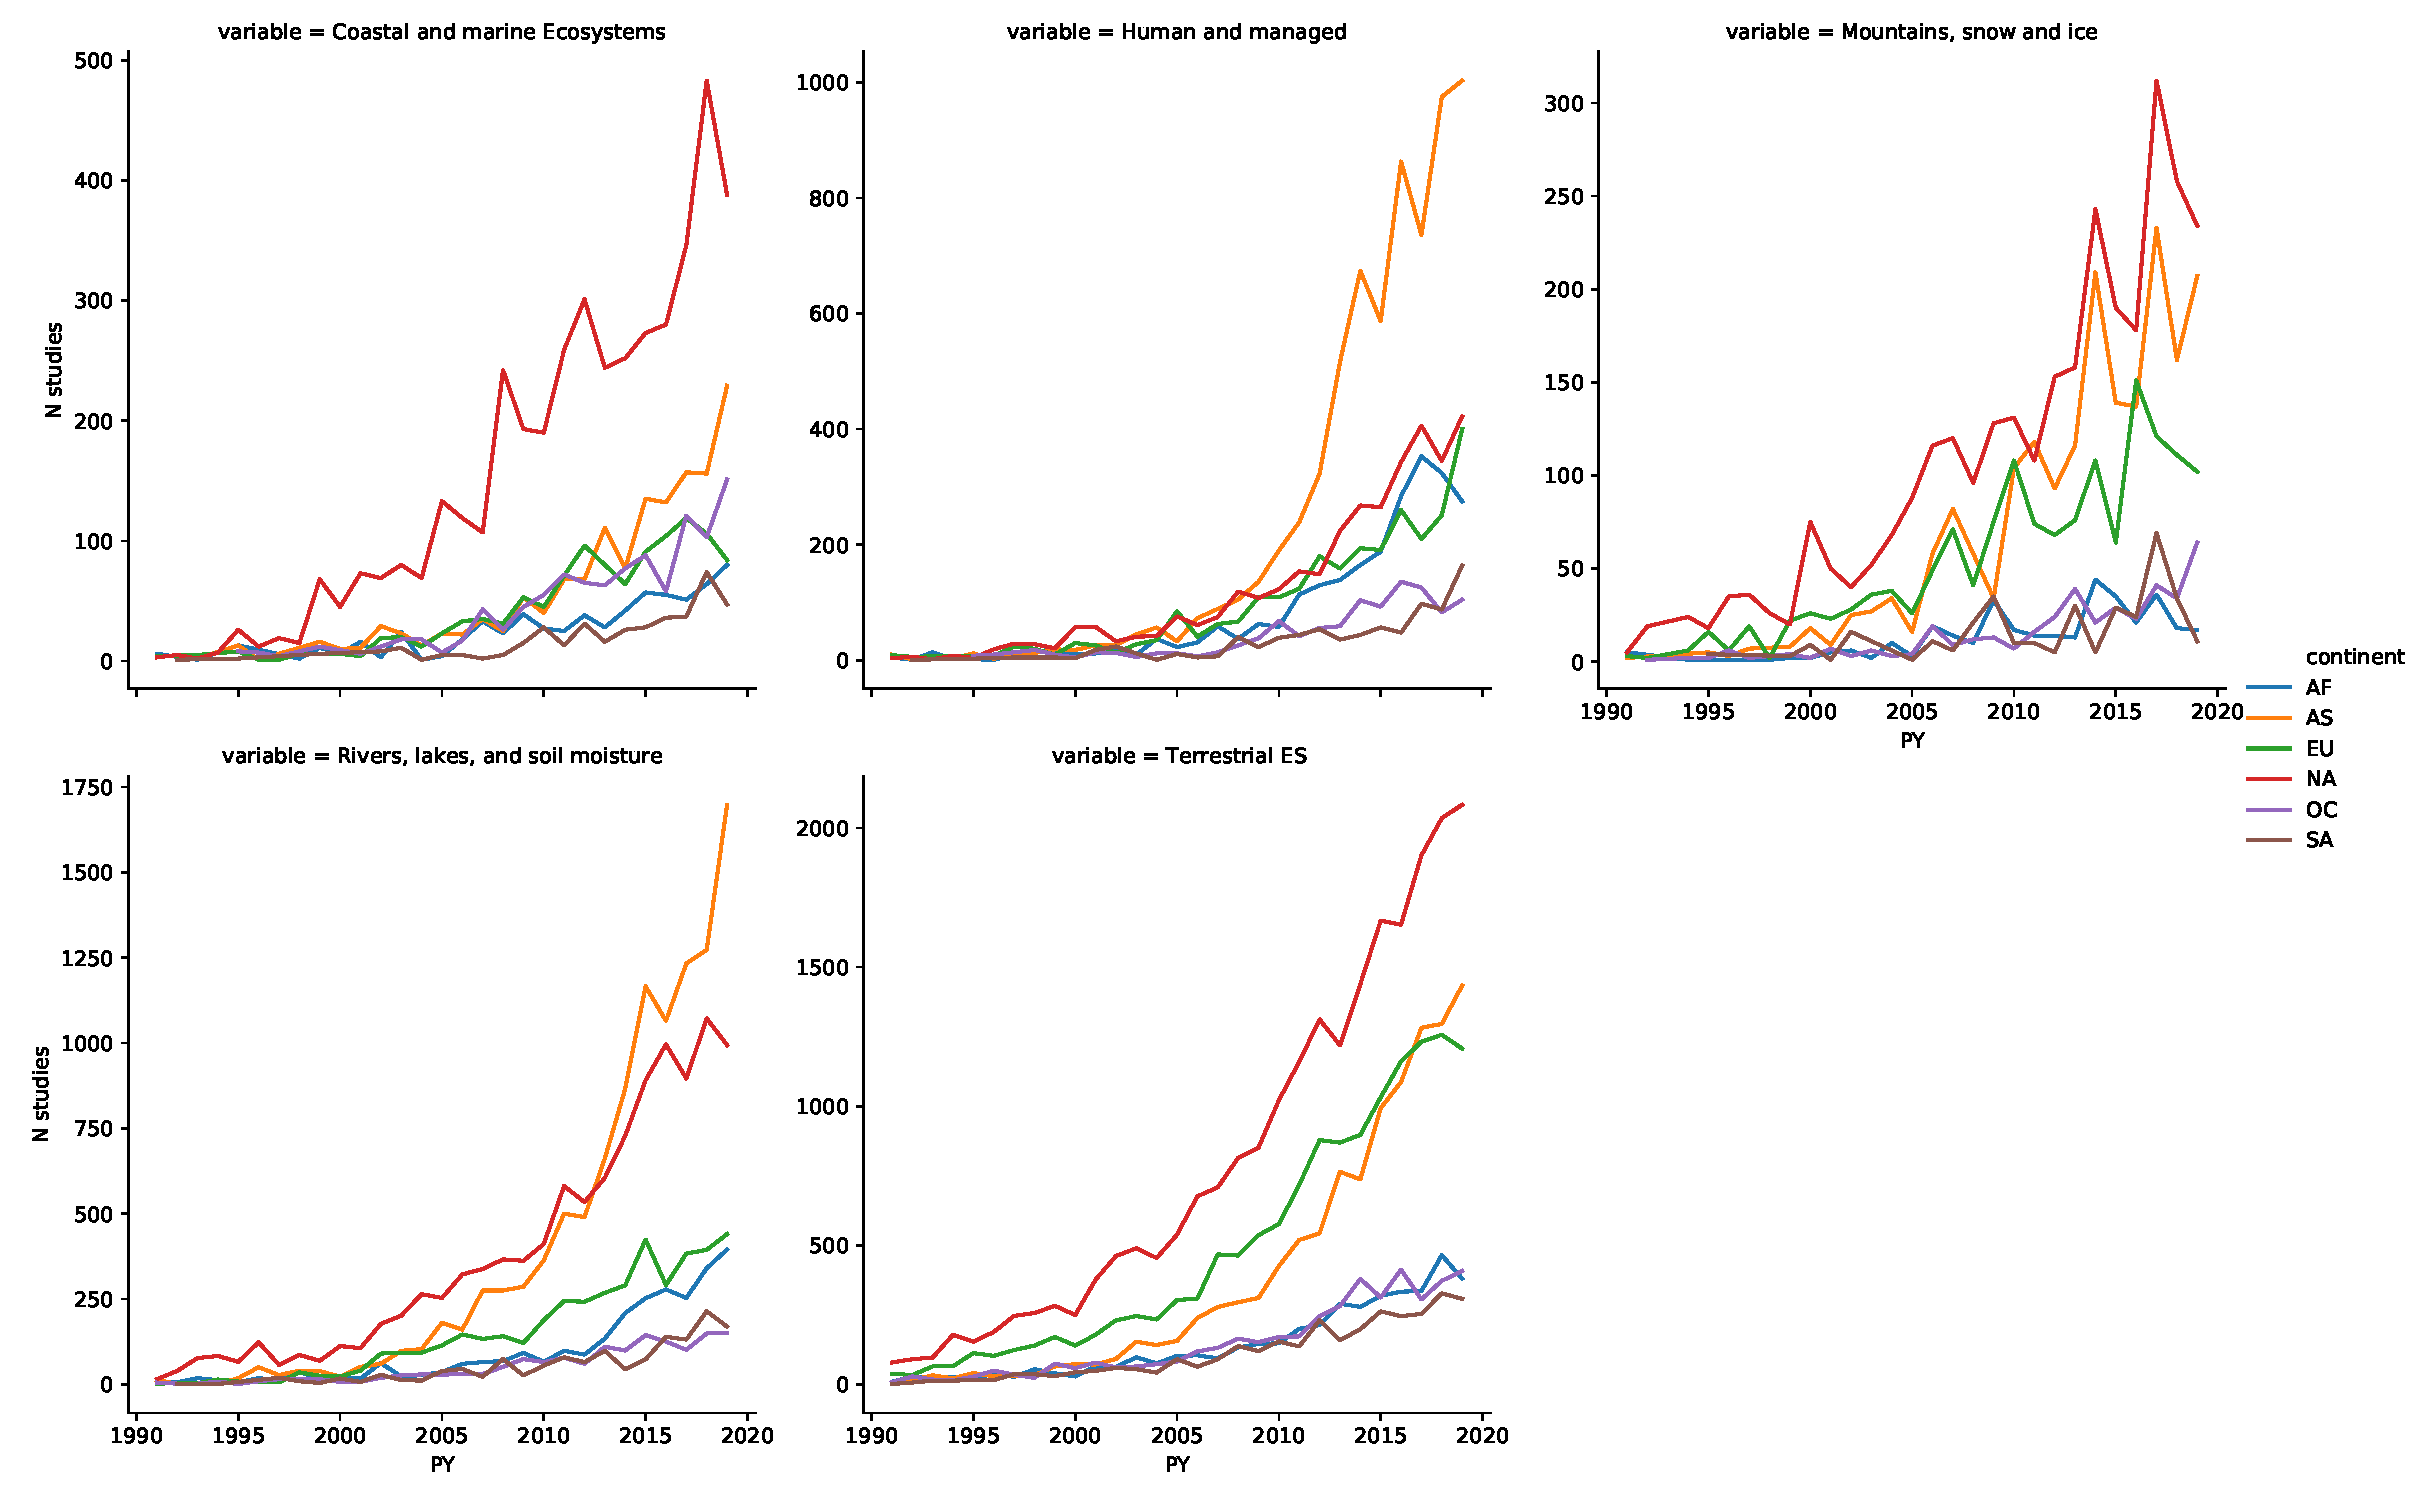
\includegraphics[width=\linewidth]{../plots/literature_distribution/PY_continent_impact.pdf}}
	
\end{column}
\end{columns}

\end{frame}

\begin{frame}{Study types}

\begin{columns}
	\begin{column}{0.618\linewidth}
		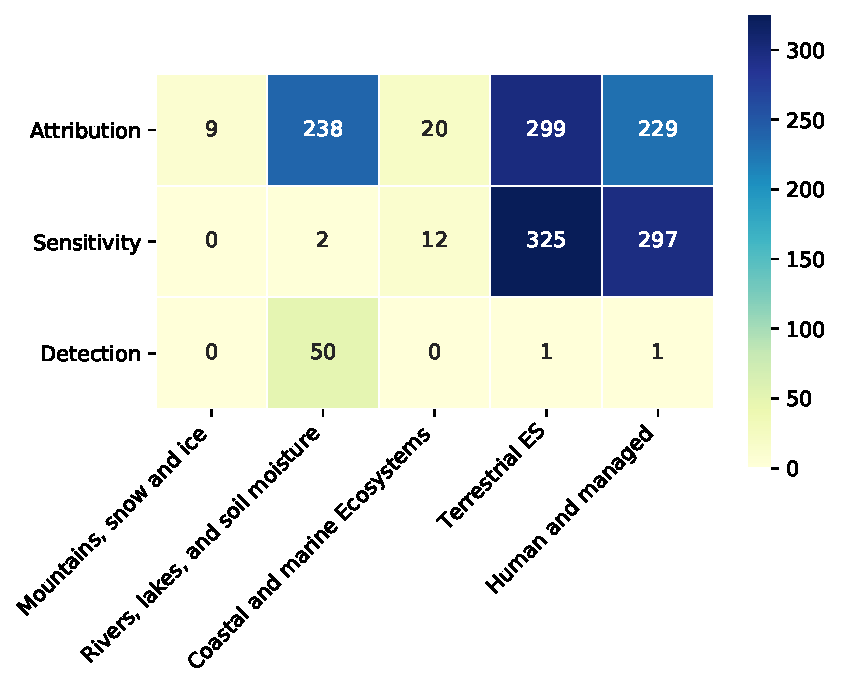
\includegraphics[width=\linewidth]{../plots/literature_distribution/heatmap_study_types_africa.pdf}
	\end{column}
	\begin{column}{0.382\linewidth}
		\begin{itemize}
			\item Most literature is on terrestrial ecosystems
			\item There's also a lot of attribution, as well as detection, literature on rivers, lakes and soil.
			\item There's a large chunk on human and managed systems, although the majority examines sensitivity rather than attribution
		\end{itemize}
	\end{column}
\end{columns}

\end{frame}

\begin{frame}{Combining data with climate models }

\begin{columns}
	\begin{column}{0.618\linewidth}
		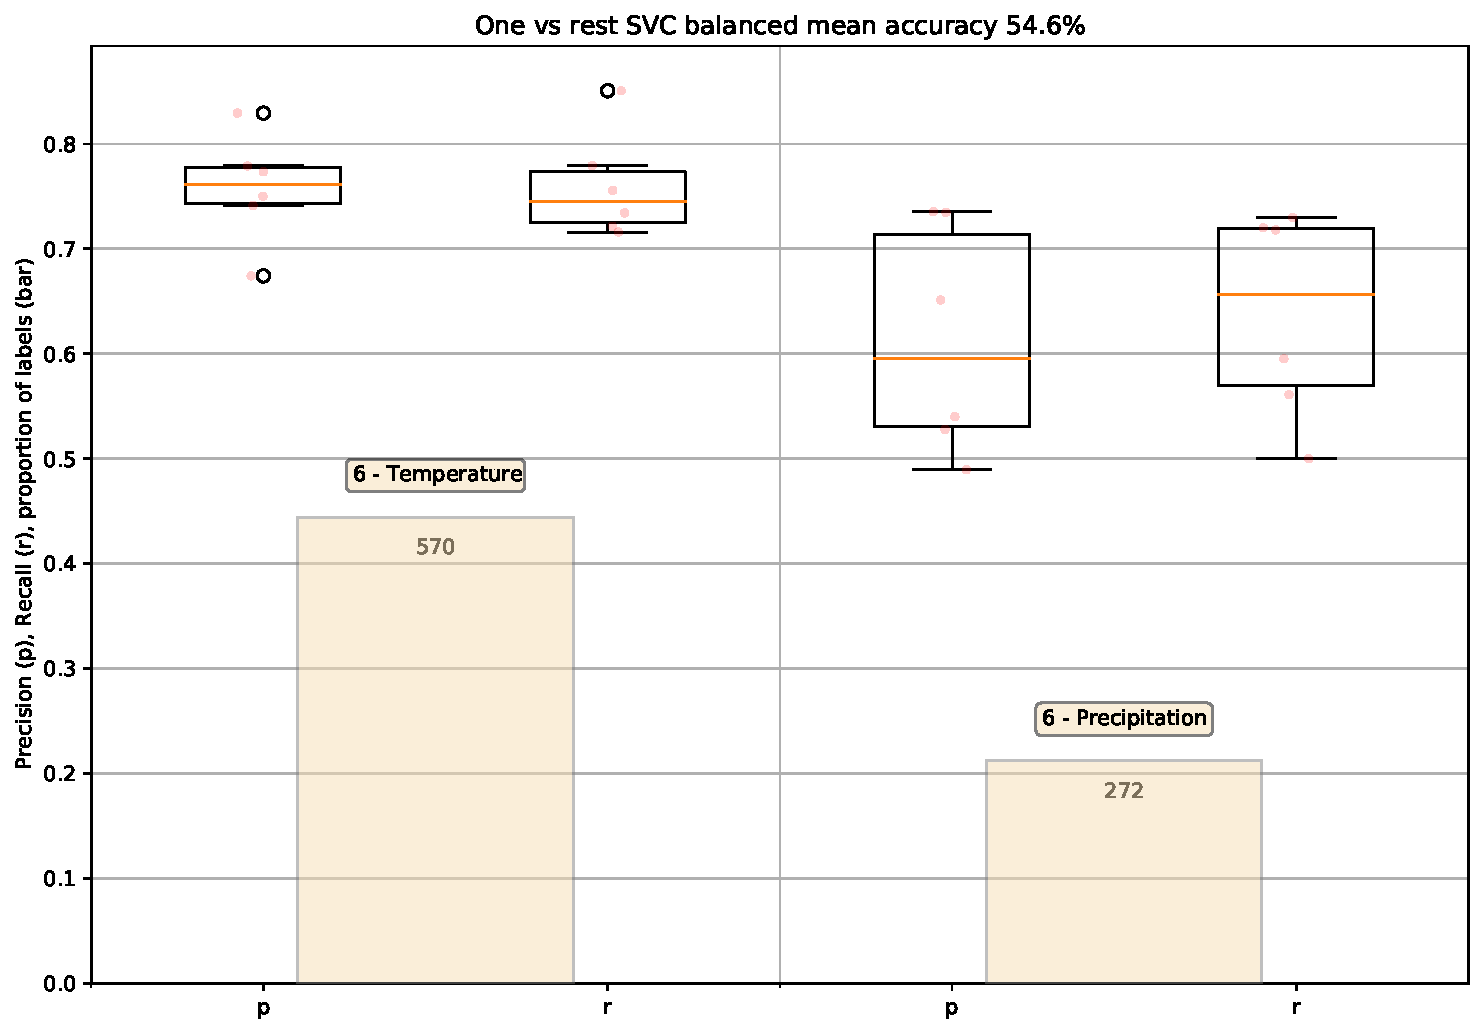
\includegraphics[width=\linewidth]{../plots/prediction_models/drivers_tp.pdf}
	\end{column}
	\begin{column}{0.382\linewidth}
		\begin{itemize}
			\item Not many papers do \textit{Full Attribution}: Human influence -> changes in regional climate variables -> regional impacts
			\item But human fingerprints on the climate are now everywhere \citep{Sippel2020}
			\item By combining our results with climate model data, we can show where impacts might be driven by anthropogenic climate change. 
		\end{itemize}
	\end{column}
\end{columns}

\end{frame}

\begin{frame}{Combining data with climate models }

	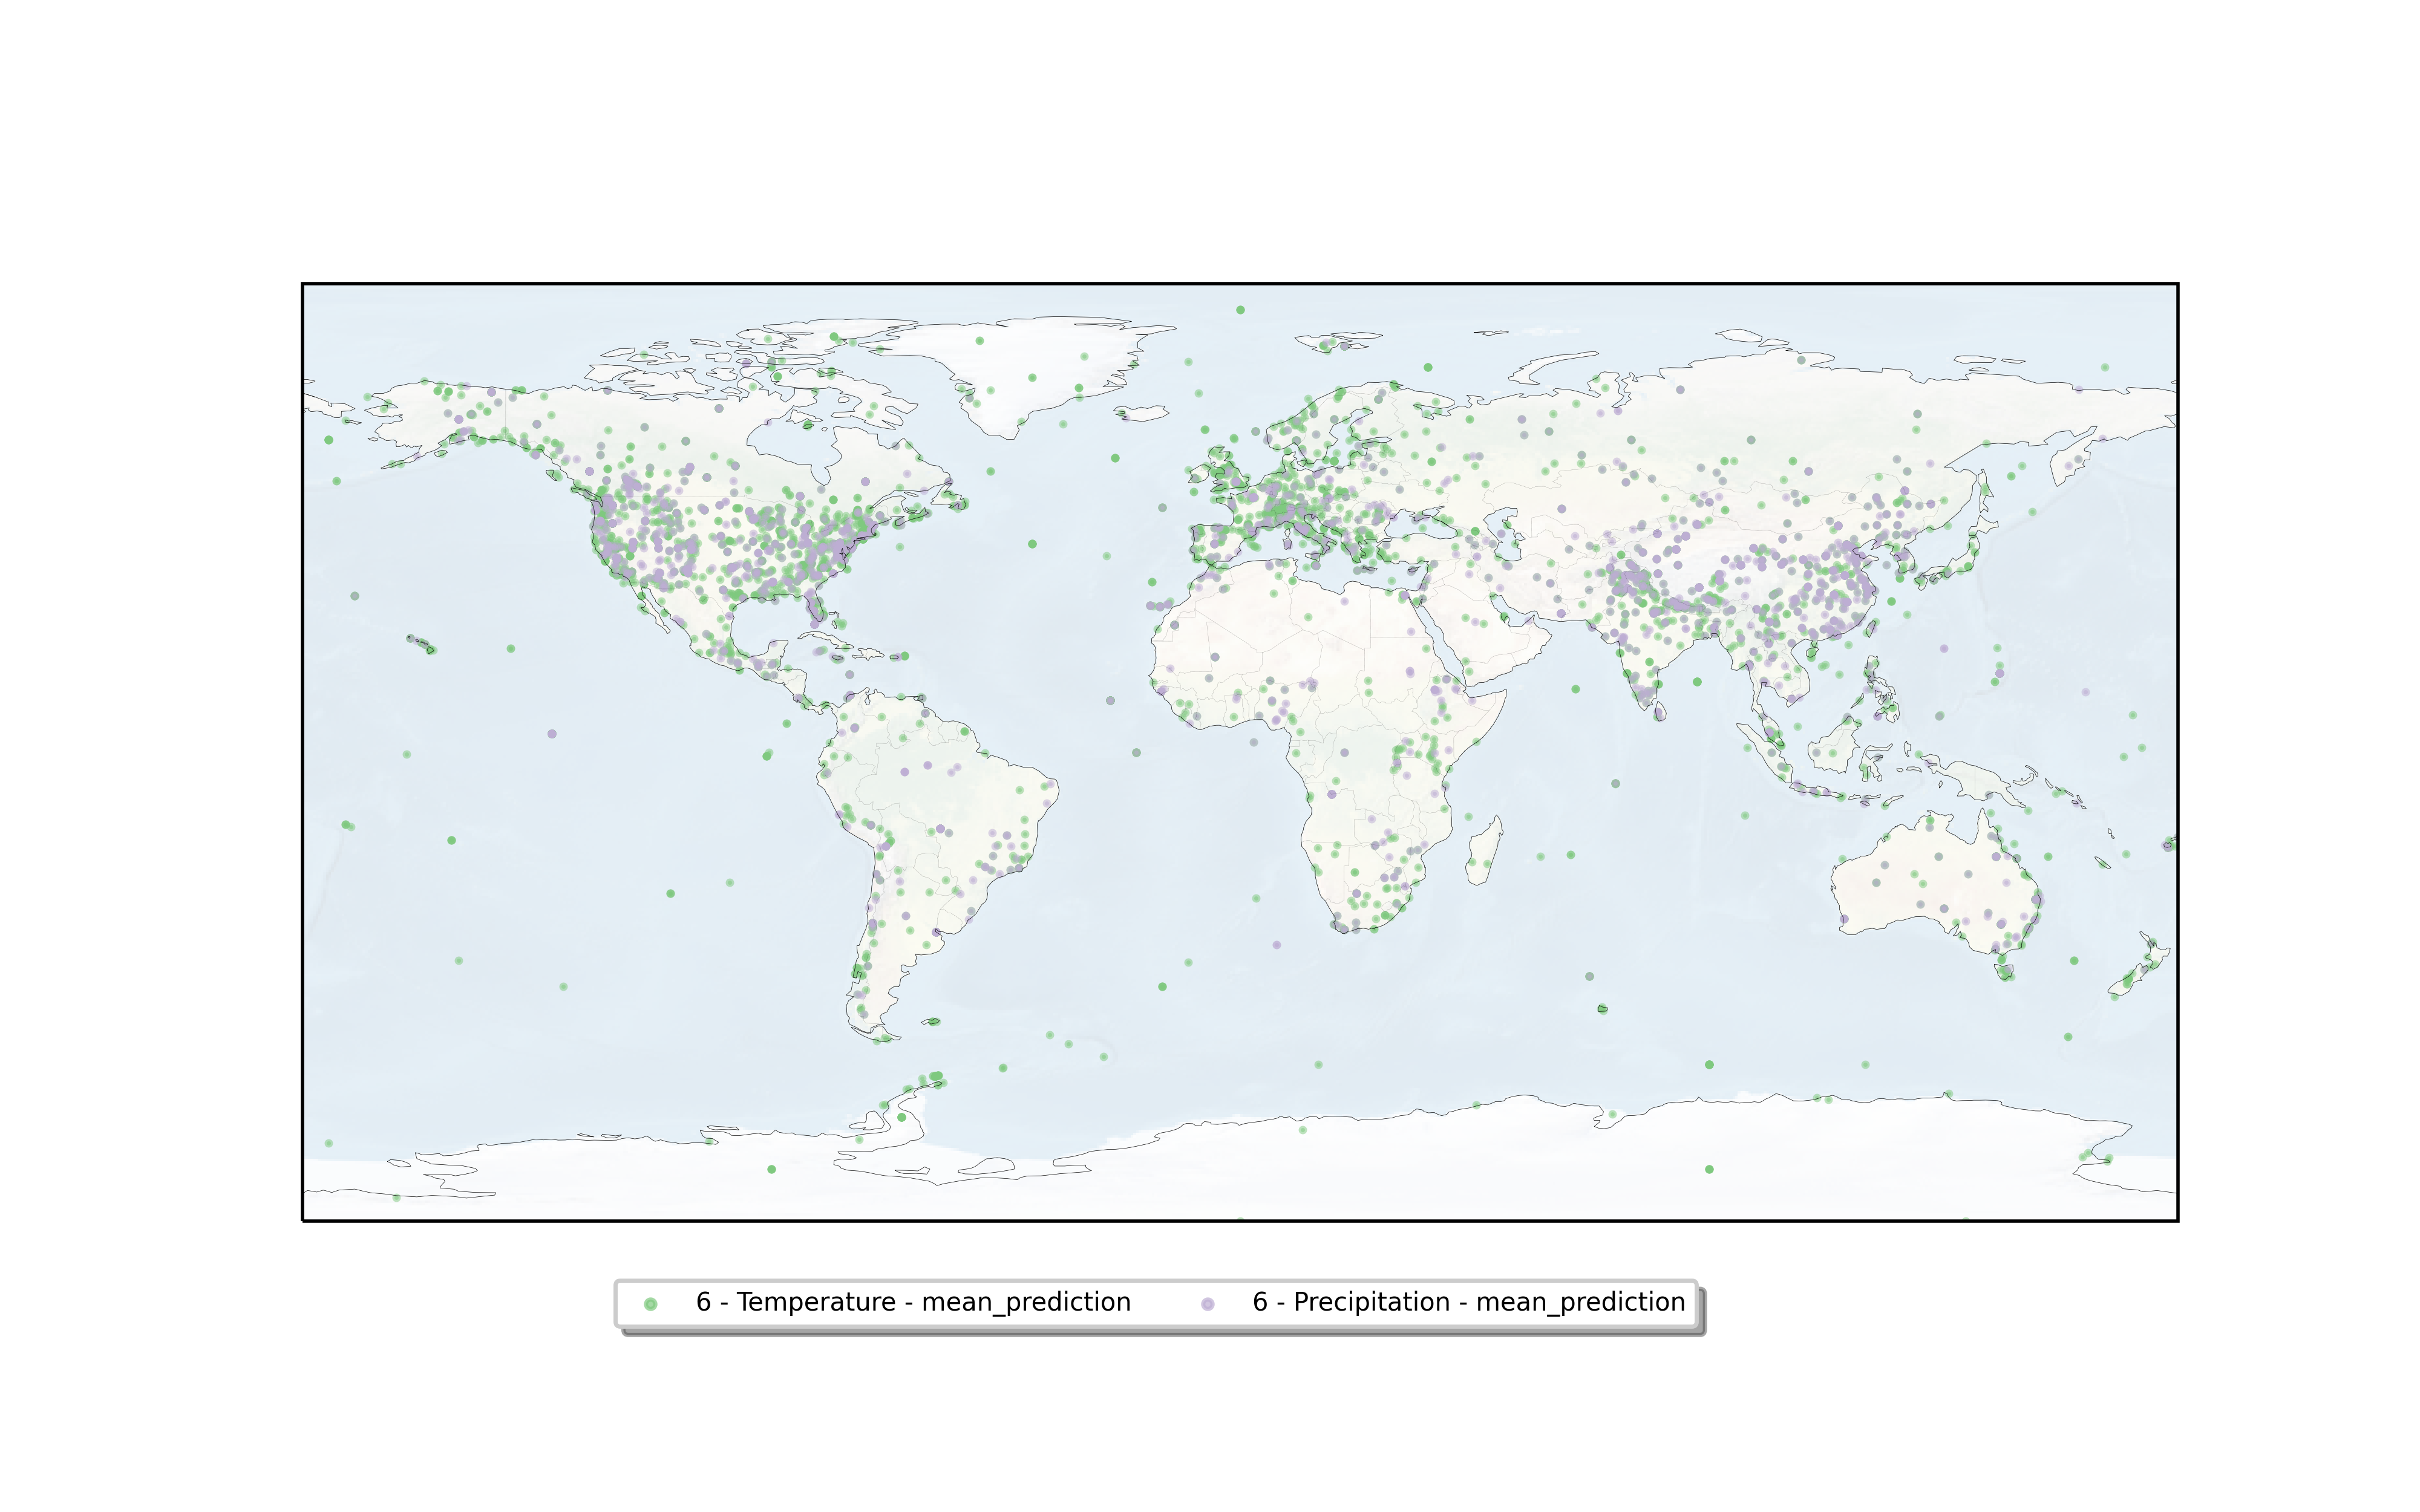
\includegraphics[width=\linewidth]{../plots/maps/predicted_places_drirvers_attribution.png}

\end{frame}



\begin{frame}{Outlook}
\begin{columns}[t]
	\begin{column}{0.5\linewidth}
		\textbf{So far}
		
		\begin{itemize}
			\item Data collection
			\item Coding scheme
			\item Coding
			\item Learning and predictions
			\item Collation of results
		\end{itemize}
	\end{column}
	\begin{column}{0.5\linewidth}
		\textbf{Still to come}
		\begin{itemize}
			\item Further data checking
			\item Investigating distribution of evidence and comparing with IPCC
			\item Predicting drivers and mapping driver-impact pathways
			\item Write up
			\item Interactive map
		\end{itemize}
	\end{column}
\end{columns}
\end{frame}


\begin{frame}{References}
\bibliography{../mendeley}
\end{frame}


\end{document}